\documentclass[12pt]{report}
\usepackage{amssymb}
\usepackage{multicol}
\usepackage{graphicx}
\usepackage{subfigure}
\usepackage{verbatim}
\usepackage[letterpaper,left=1cm,right=2cm, top=1.5cm,
bottom=1.5cm,head=0cm,foot=1cm]{geometry}

\parindent=0in


\newcommand{\m}{\mbox{ m }}
\newcommand{\kg}{\mbox{ kg }}
\newcommand{\s}{\mbox{ s }}
\newcommand{\ke}{\mbox{\small KE}}
\newcommand{\pe}{\mbox{\small PE}}


\newcommand{ \probDir}[1]{{ \bf\small #1 \mbox{  }}}

\newcommand{ \breakList}{\setcounter{saveenum}{\value{enumi}} \end{enumerate}}
\newcommand{ \contList}{\begin{enumerate} \setcounter{enumi}{\value{saveenum}}}

\newcounter{saveenum}

\def \wspace{5cm}

%%%%%%%%%%%%%%%%%%%%%%%%%%%%%%%%%%%%%%%%%
\begin{document}

{\bf{Honors Physics} \hfill {Quiz 3: Momentum and Mechanical Energy} \hfill {Mr. Kelley}} \\ \\
%%%%%%%%%%
$\rho=mv$ \hfill $\ke=\frac{1}{2}mv^2$ \hfill $\pe=mgh$ \hfill $\rho_\circ = \rho_f$ \hfill $\ke_\circ + \pe_\circ = \ke_f + \pe_f$


\begin{enumerate}
\item A skateboarder with a mass of 60 kg is skating on perfectly frictionless bearings (and wheels) at a speed of 22 m/s.  A 10 kg puppy falls out of the sky, directly into the skateboarder's arms.  How fast is the puppy-skater now moving?
\vfill
\item A tennis ball hits a duck head-on.  The duck was flying with a speed of 5 m/s, and the tennis ball was traveling with a speed of 18 m/s.  If the tennis ball bounces straight back (reverses direction) with a speed of 4 m/s, how fast is the duck now going?  The duck has a mass of 1 kg and the tennis ball 57 g.  (Hint: UNITS! SIGNS!)
\vfill
\pagebreak
\item Slightly dazed, the duck flies into the side of a building 20 m above the ground and comes to a stop, then falls towards the earth.  How fast will the duck be going when it reaches ground level?  (Neglect air resistance.)
\vfill
\item It turns out that this was a \emph{rubber} duck and it bounces straight up with an initial velocity of 16 m/s.  How high will it go?  (Neglect air resistance.)
\vfill
\pagebreak
\item A kumquat is flying through outer space at a constant speed of 10 m/s.  It hits a stationary pomelo and bounces off at 6 m/s with an angle of $20^\circ$.  What is the final velocity (magnitude and direction) of the pomelo?  The pomelo's mass is 205 g, and the kumquat's is 3 g.  Draw a picture.
\vfill
\pagebreak
\item What is the center of mass of this system?  (Hint: Choose an origin) 
$$ x_{\mbox{\tiny CM}} = \frac{\sum\limits_{i=1}^{n} m_i x_i}{\sum\limits_{i=1}^{n} m_i}$$
\begin{center}
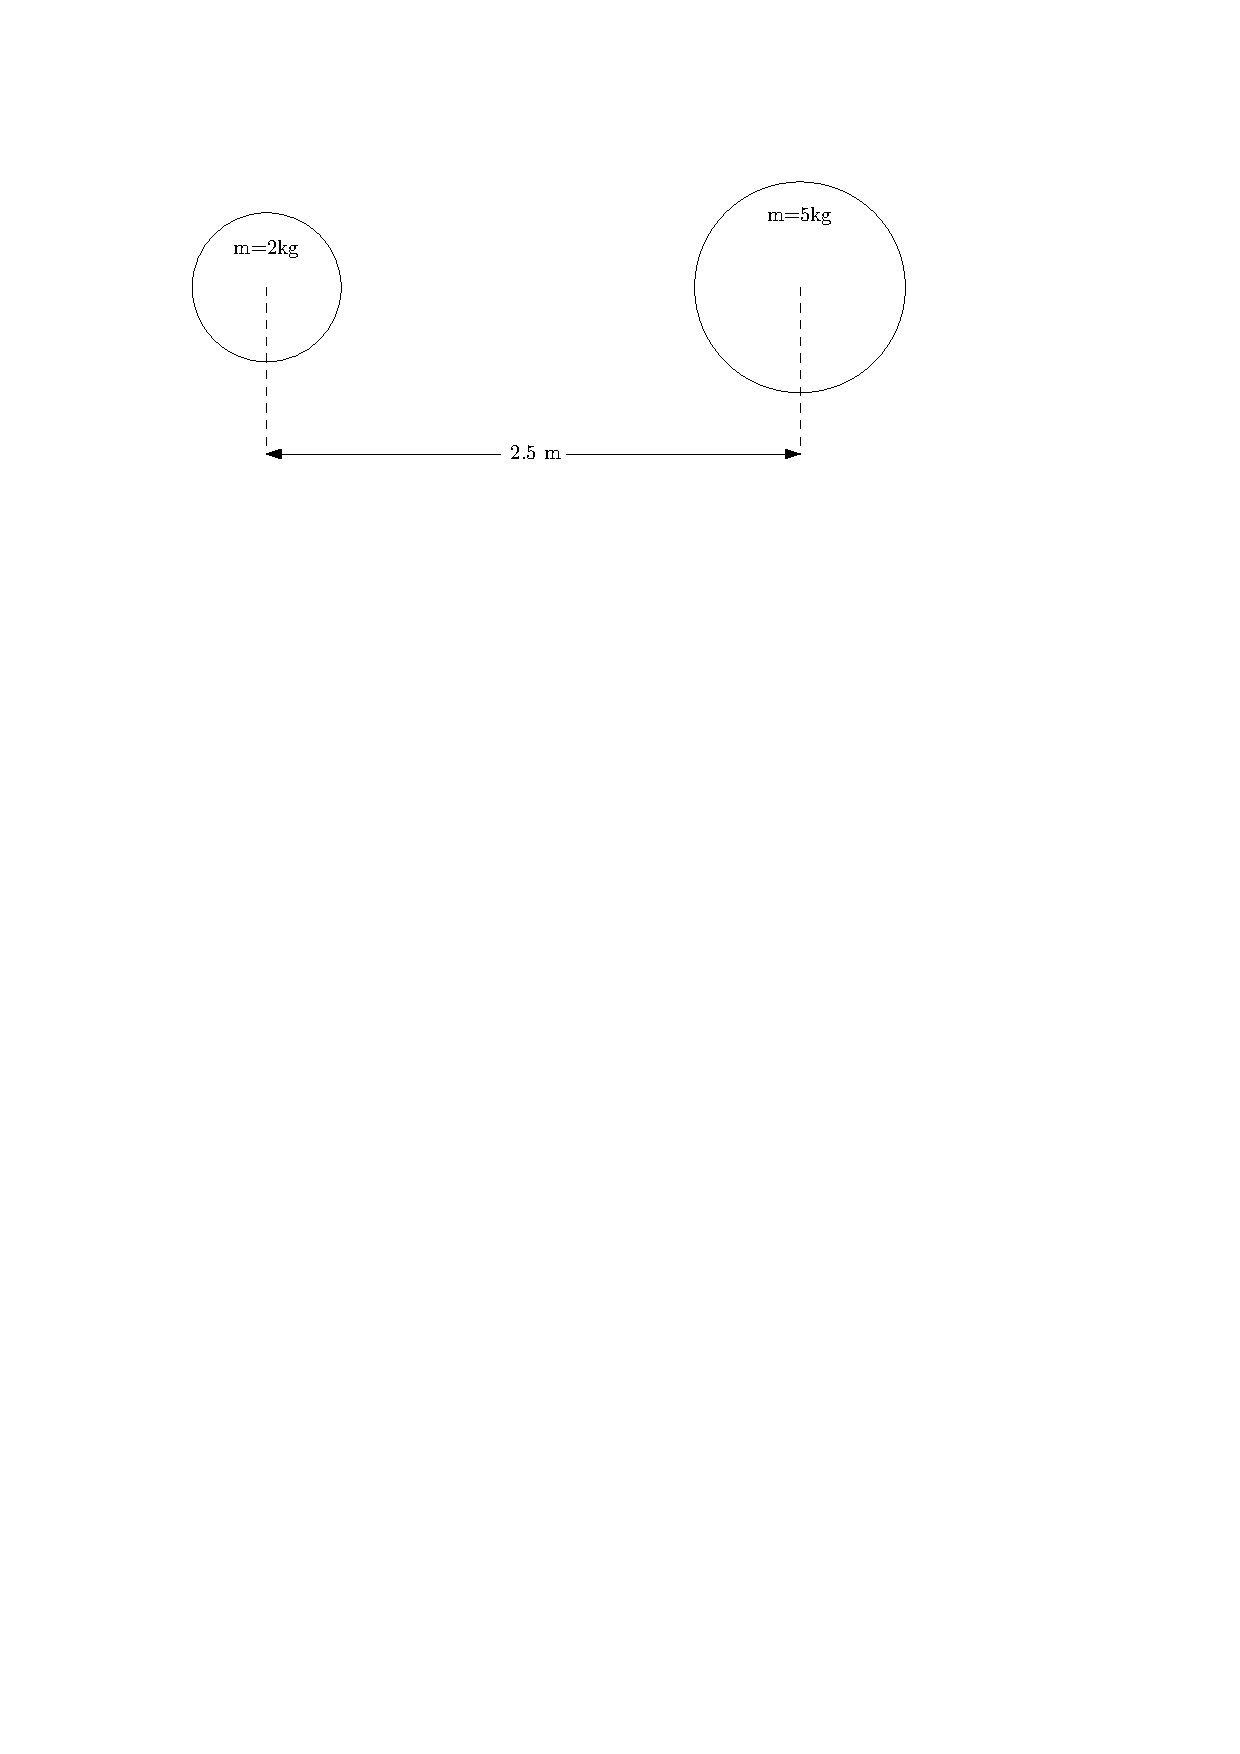
\includegraphics[ scale = 1.2]{2massCM.pdf}
\end{center}
\vfill
%%%%
\end{enumerate}




\end{document}